\section{Learned network-editor evaluation}
\label{sec:experiments}

\paragraph{Astra failure probe.} We evaluate \astra (\code{gpt-6-astra}) through the Chat Completions API at medium
reasoning effort, with a 32{,}000-token completion cap, no tools, \code{store=false} and one sample per task.
\astra works in its natural mode: it receives the drafting conventions, the physical model (fluid properties,
friction law, loss conventions) and the criteria in the prompt, and it returns the complete edited SVG followed
by a JSON analysis stating the verdict, the violating components and the governing quantities. The edited SVG
is scored by \ours exactly as any other drawing (\cref{sec:method}), and the analysis is compared with the
solver's. Tasks are the first ten test edits by identifier for every (family, edit type) pair of the main tier
(100 tasks), and the first four of the hard tier (40 tasks). The API account ran out of credit during the run.
All \astraMainN{} main-tier and \astraHardN{} hard-tier tasks that completed are reported. Every circuit task
completed. The missing tasks are all pipe networks, which failed with ``no credits remaining'' (26) or a
dropped connection (12), and they are excluded rather than counted as failures.

\paragraph{Our editor.} \ours pairs the verifier with a small editor: Qwen2.5-Coder-Instruct~\cite{hui2024qwen25coder}
at 1.5B and 7B parameters, fine-tuned with LoRA~\cite{hu2022lora} (rank 16 on the attention projections) for two
epochs on the \netEdits{}-edit training split to map \emph{source SVG $+$ instruction} to a tree patch. The patch
is applied by a validating executor, and the resulting drawing is recovered and solved, so the verdict is
computed, not generated. Decoding is greedy. The hard tier is never seen in training. We compare two ways for
a patch to name the elements it changes. \emph{Positional} addressing uses the executor's native node
identifiers, where \code{n77} is the 77th element in document order. \emph{Id} addressing uses the element's own
SVG identifier (\code{\#R5-label}) and writes insertion at the end of a group as \code{"end"}. It is
translated to positional form before execution, so the two differ only in what the model must write.

\paragraph{Metrics.} \emph{Edit}: the edited drawing recovers to the target network. \emph{Verdict}: the stated
pass/fail matches the solver's. \emph{Violations}: the set of violating components matches exactly. \emph{All}: all
three at once. For systems whose verdict is computed by \ours, the verdict is taken from the solve of the edited
drawing, whether or not the edit was correct.

\begin{table*}[t]
\centering
\footnotesize
\setlength{\tabcolsep}{5pt}
\begin{tabular}{lcccc}
\toprule
System & Edit & Verdict & Violations & All \\
\midrule
\multicolumn{5}{l}{\textbf{Main tier} (same completed tasks for every system)} \\
\compareMainRows
\midrule
\multicolumn{5}{l}{\textbf{Hard tier} (8--16 loops for circuits; unseen in training)} \\
\compareHardRows
\bottomrule
\end{tabular}
\caption{\textbf{Edit and verdict accuracy}, \% (count), on the tasks \astra completed. ``\astra drawing $+$
\ours verdict'' keeps \astra's edited SVG but replaces its analysis with the solve of that drawing.}
\label{tab:compare}
\end{table*}

\subsection{Control cases and failure context}
\astra is an accurate editor of these drawings. Every one of its completed edits recovers to the target
network, including parallel branches drawn as tapped sub-circuits and pipes added between junctions, and it
never disconnected a wire or broke the drafting conventions. Its circuit analysis is exact on every
completed task, including hard-tier networks with up to 16 independent loops. We did not find the failure
boundary we expected for linear networks: at these sizes, unaided nodal analysis is within reach. Each answer
costs \$\astraMainCost{} on the main tier and \$\astraHardCost{} on the hard tier on average, and takes a median
of \astraMainSeconds{}\,s and \astraHardSeconds{}\,s respectively, with no truncated responses.

\subsection{Astra's silent wrong verdict}
\begin{figure}[t]
\centering
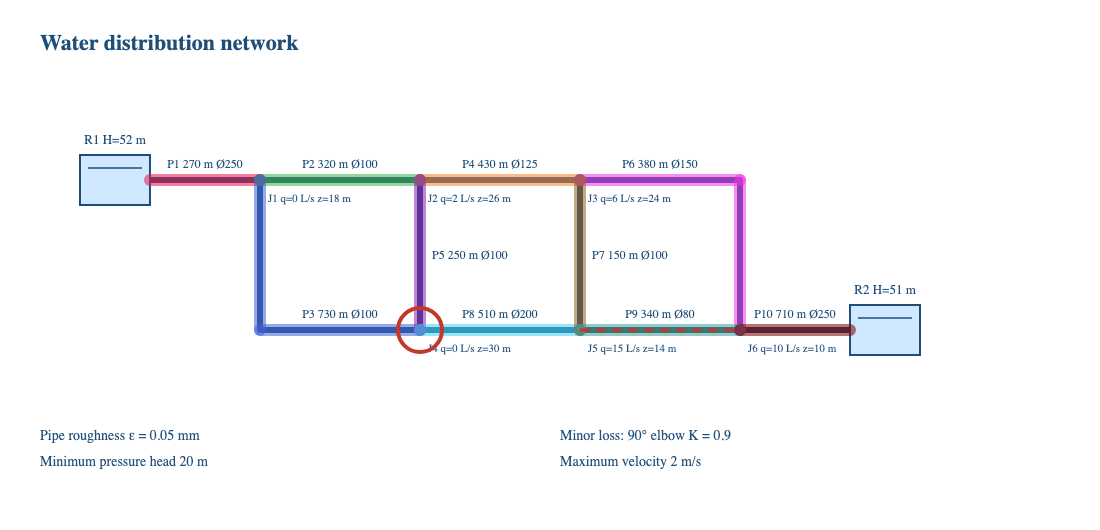
\includegraphics[width=\linewidth,trim=60 150 160 120,clip]{figures/astra-failure-pipe.png}
\caption{\textbf{Astra's wrong verdict on its edited SVG.} ``Change the length of P9 to 340\,m'' (dashed) in a two-reservoir
network with four loops. \astra's edit is correct, and it reports the minimum pressure head at J4 (circled) as
20.04\,m and the design as passing. Re-solving the drawing gives 19.23\,m, below the 20\,m minimum stated on
the drawing. Several of its pipe velocities are off by up to 67\,\%.}
\label{fig:failure}
\end{figure}

The only substantive error among \astra's completed network answers is in a nonlinear pipe network, and it is not flagged
(\cref{fig:failure}). The edit is right, but the analysis declares a failing design safe: it reports 20.04\,m
of pressure head where the drawing yields 19.23\,m against a 20\,m minimum, and its flows are wrong
throughout the loop that contains the edited pipe. Nothing in the answer
distinguishes it from the correct ones: it finished normally, used a similar reasoning budget, and presented
its numbers with the same precision. This is the failure mode a verifier exists for. It is rare (1 of
\astraMainN{} main-tier answers), it concentrates where the physics is nonlinear and the design sits near a
limit, and it cannot be detected from the answer itself. Replacing \astra's analysis with the solve of its
own drawing removes it (\cref{tab:compare}, second row). The source drawing already puts J4 below the 20\,m
limit (19.26\,m); the P9 edit leaves it below that limit (19.23\,m). \Cref{fig:astra-worked} shows both
drawings and the saved answer in detail.

\subsection{The small editor}
\begin{figure}[t]
\centering
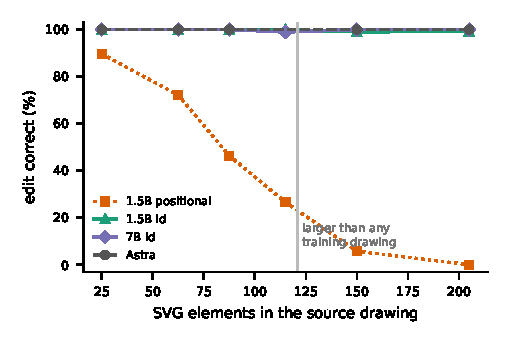
\includegraphics[width=\linewidth]{figures/size-curve.pdf}
\caption{\textbf{Edit accuracy against drawing size}, pooled over both tiers and binned by the number of SVG
elements in the source drawing (bins with at least five edits). The grey line marks the largest drawing in
the training split.}
\label{fig:size}
\end{figure}
\oursDiscussion

\begin{table}[t]
\centering
\scriptsize
\setlength{\tabcolsep}{1.8pt}
\begin{tabular}{@{}lccc@{}}
\toprule
Editor & Circuits & Pipes & All \\
\midrule
\oursFullRows
\bottomrule
\end{tabular}
\caption{\textbf{Our editor on the full test sets}: edit correctness by family and end-to-end accuracy (``pos.'' = positional, ``id'' = id addressing) on all 1{,}000 main-tier and \hardEdits{} hard-tier edits, \% (count).}
\label{tab:ours}
\end{table}

\subsection{Cost of a verified edit}
\costDiscussion
